% The first segment of the shop built from the Hitting Set instance U = {1,2,3}, F_1 = {2,3},
% F_2 = {1,2}, F_3 = {1,3}, k = 2, drawn to scale: the unit is Q = (k-1)(n+1) = 4, the three epochs
% have lengths 3Q, 5Q and 7Q, and the jobs of element i are shifted by i = Q * (i/4).
% Adapted from the construction figure of the paper.
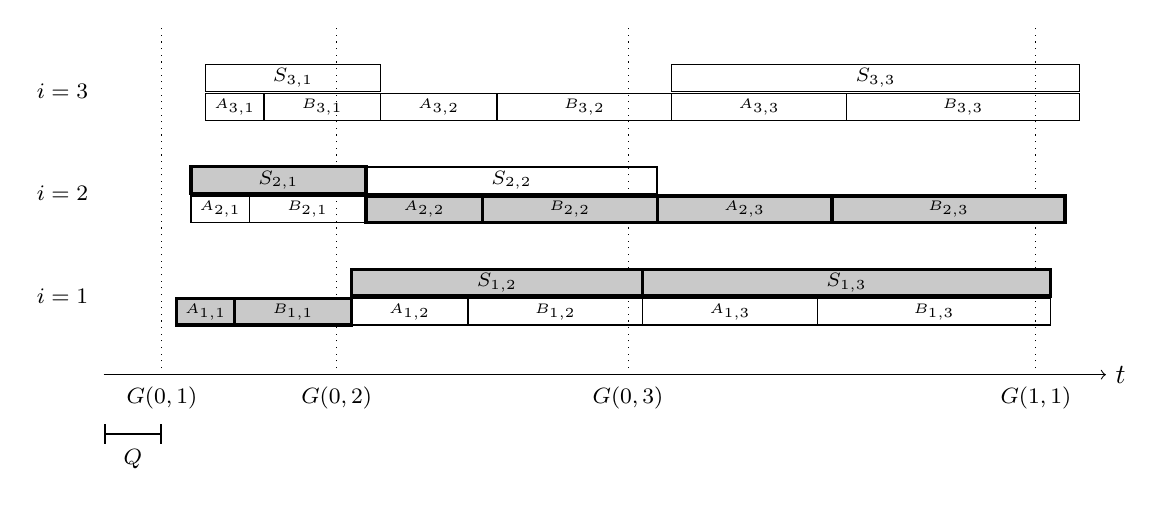
\begin{tikzpicture}[x=0.74cm,y=1cm]
\def\h{0.17}
\colorlet{sel}{gray!42}
\tikzset{job/.style={draw,line width=0.5pt},
         chosen/.style={draw,fill=sel,line width=1.2pt}}

% the epoch boundaries G(0,1) = Q, G(0,2) = 4Q, G(0,3) = 9Q, G(1,1) = 16Q
\foreach \g/\lab in {1/{G(0,1)}, 4/{G(0,2)}, 9/{G(0,3)}, 16/{G(1,1)}}
{
    \draw[dotted] (\g,-0.55) -- (\g,3.85);
    \node[font=\footnotesize] at (\g,-0.85) {$\lab$};
}
\draw[->] (0,-0.55) -- (17.2,-0.55) node[right] {$t$};
\draw[|-|,line width=0.8pt] (0,-1.3) -- (1,-1.3);
\node[font=\footnotesize] at (0.5,-1.62) {$Q$};

% rows: element i = 1, 2, 3 (bottom to top); a selection job S_{i,j} lies above two dummies A, B
\foreach \i in {1,2,3}
{
    \pgfmathsetmacro{\yD}{(\i-1)*1.3+0.25}
    \pgfmathsetmacro{\yS}{(\i-1)*1.3+0.62}
    \pgfmathsetmacro{\sh}{\i/4}
    \node[anchor=east,font=\footnotesize] at (-0.1,\yD+0.2) {$i=\i$};
    \foreach \j/\g/\gn in {1/1/4, 2/4/9, 3/9/16}
    {
        \pgfmathsetmacro{\xa}{\g+\sh}
        \pgfmathsetmacro{\xm}{\g+\j+\sh}
        \pgfmathsetmacro{\xb}{\gn+\sh}
        \draw[job] (\xa,\yD-\h) rectangle (\xm,\yD+\h) node[midway,font=\tiny] {$A_{\i,\j}$};
        \draw[job] (\xm,\yD-\h) rectangle (\xb,\yD+\h) node[midway,font=\tiny] {$B_{\i,\j}$};
    }
}
% selection jobs: S_{i,j} exists when i is in F_j
\foreach \i/\j/\g/\gn in {1/2/4/9, 1/3/9/16, 2/1/1/4, 2/2/4/9, 3/1/1/4, 3/3/9/16}
{
    \pgfmathsetmacro{\yS}{(\i-1)*1.3+0.62}
    \pgfmathsetmacro{\sh}{\i/4}
    \draw[job] (\g+\sh,\yS-\h) rectangle (\gn+\sh,\yS+\h) node[midway,font=\scriptsize] {$S_{\i,\j}$};
}
% the schedule of the hitting set H = {1,2}, in gray
\foreach \i/\j/\g/\gn in {2/1/1/4, 1/2/4/9, 1/3/9/16}
{
    \pgfmathsetmacro{\yS}{(\i-1)*1.3+0.62}
    \pgfmathsetmacro{\sh}{\i/4}
    \draw[chosen] (\g+\sh,\yS-\h) rectangle (\gn+\sh,\yS+\h) node[midway,font=\scriptsize] {$S_{\i,\j}$};
}
\foreach \i/\j/\g/\gm/\gn in {1/1/1/2/4, 2/2/4/6/9, 2/3/9/12/16}
{
    \pgfmathsetmacro{\yD}{(\i-1)*1.3+0.25}
    \pgfmathsetmacro{\sh}{\i/4}
    \draw[chosen] (\g+\sh,\yD-\h) rectangle (\gm+\sh,\yD+\h) node[midway,font=\tiny] {$A_{\i,\j}$};
    \draw[chosen] (\gm+\sh,\yD-\h) rectangle (\gn+\sh,\yD+\h) node[midway,font=\tiny] {$B_{\i,\j}$};
}
\end{tikzpicture}
